\section{Dynamic Systems}

A dynamic system is a system that evolves during time. Until now, we didn't consider time. Now we will consider a system that also considers time and, in particular, discrete time.

\begin{figure}[H]
    \centering
    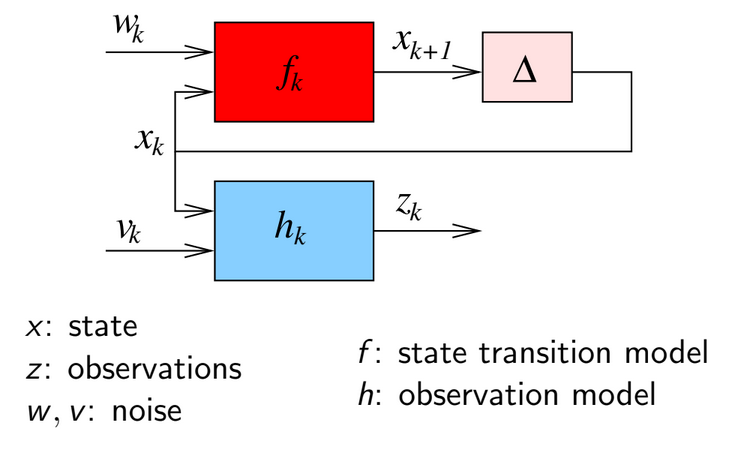
\includegraphics[width=12cm]{images/Reinforcement Learning/dynam_sys.png}
    \caption{Taxonomy ao a dynamic system}
    \label{fig:dyn_sys}
\end{figure}

An important step in the dynamic system \ref{fig:dyn_sys} is $X_{k}$ which is the snapshot f how is the situation at this moment, while $X_{k + 1}$ is the snapshot at the next timestep. The evolution can be represented by a list of snapshots: $X_{1}, X_{2}, \dots, X_{t}$. The state transmission model $f_{k}$ is the function that evolves the system. This function models how the state changes between steps. In this picture, the input variables that influences this function are not shown. However they are implicitly represented inside the noise $W_{k}$. We have another important model which is the observation model $h_{k}$. $z_{k}$ are the observations created by the observation model. $\Delta$ is an offset in time that gives to the model consideration of time.

\subsection{Reasoning vs learning in Dynamic Systems}
For \textbf{reasoning}, we have the model $(f, h)$ (Input) and the current state $x_{k}$, so we can predict the future $(x_{k + T}, z_{k + T})$. In \textbf{learning} we have the past experience $(z_{0:k})$ (Input) and we want to determine the model $(f, h)$.

\subsection{State of a Dynamic System}

The staet $x$ encodes:
\begin{itemize}
    \item all the past knowledge needed to predict the future
    \item the knowledge gathered through operation
    \item the knowledge needed to pursue the goal
\end{itemize}

When the state is fully observable, the decision making problem for an agent is to decide which action must be executed in a given state. The agent has to compute the function:
\begin{equation}
    \pi : X \xrightarrow{} A
\end{equation}
The goal of the agent is to learn a function $\pi$ that maps states to actions.

If we want to compare Reinforcement Learning and Supervised learning, we can point out that:
\begin{itemize}
    \item Supervised learning tries to learn a function $f : X \xrightarrow{} Y$, given $D = \{x_{i}, y_{i}\}$
    \item Reinforcement learning tries to learn a function $\pi : X \xrightarrow{} A$, given\\ 
    $D = \{ \langle (x_{1}, a_{1}, r_{1}), \dots, (x_{n}, a_{n}, r_{n}) \rangle \}^{(i)}$
\end{itemize}
where $x_{i}$ is the $i$-th state, $a_{i}$ is the $i$-th action and $r_{i}$ is the $i$-th reward. Notice that in a RL dataset we have any combination of states, actions and rewards.

\subsection{Dynamic System Representation}

$X$: set of states
\begin{itemize}
    \item \textbf{explicit discrete and finite representation} $X = \{x_{1}, \dots, x_{n}\}$
    \item continuous representation $X = F(\dots)$ (state function)
    \item probabilistic representation $P(X)$ (probabilistic state function)
\end{itemize}
$A$: set of actions
\begin{itemize}
    \item \textbf{explicit discrete and finite representation} $A = \{xa_{1}, \dots, a_{n}\}$
    \item continuous representation $A = U(\dots)$ (control function)
\end{itemize}
$\delta$: transition function
\begin{itemize}
    \item deterministic / non-deterministic / \textbf{probabilistic}
\end{itemize}
$Z$: set of observations
\begin{itemize}
    \item explicit discrete and finite representation $Z = \{xz_{1}, \dots, z_{n}\}$
    \item continuous representation $Z = \zeta(\dots)$ (observation function)
    \item probabilistic representation $P(Z)$ (probabilistic observation function)
\end{itemize}

\subsection{Markov property}

The Markov property states that: 
\begin{itemize}
    \item Once the \textbf{current state is known}, the evolution of the dynamic system does \textbf{not depend} on the \textbf{history} of states, actions and observations.
    \item The \textbf{current state contains all the information needed} to predict the future.
    \item \textbf{Future} states are \textbf{conditionally independent} of past states and past observations given the current state.
    \item The knowledge about the current state makes past, present and future observations statistically independent.
\end{itemize}

A Markov process is a process that has the Markov property

\subsection{Markov Decision Process (MDP)}
Markov processes for decision making. \\
States are fully observable, no need of observations. \\
Graphical model:

\begin{figure}[H]
    \centering
    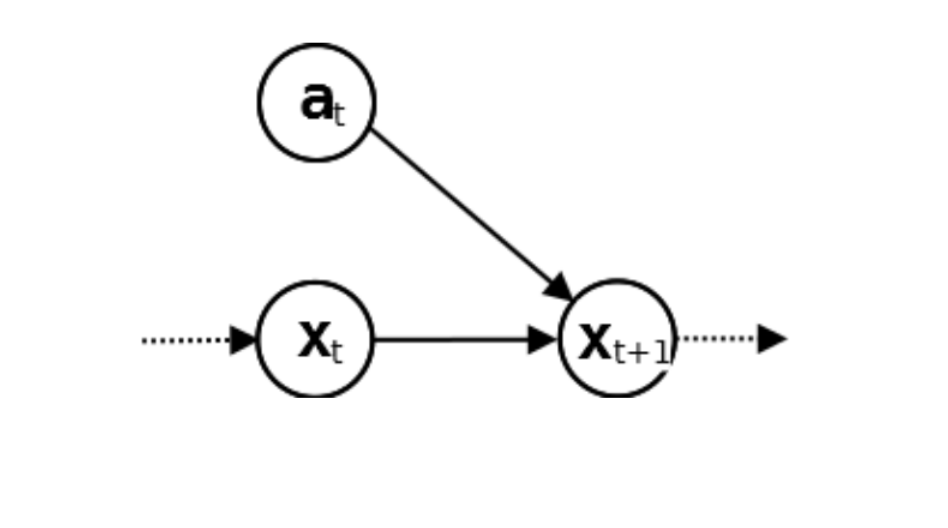
\includegraphics[width=8cm]{images/Reinforcement Learning/mdp.png}
    \caption{MDP graphical model}
    \label{fig:mdp}
\end{figure}

\section{Markov Decision Process (MDP)}
It is a decision process based on subsequent actions that makes the model evolve during time.
\subsection{Deterministic transaction}
\begin{equation}
    MDP = \langle X, A, \delta, r\rangle
\end{equation}
where $X$ is a finite set of states, $A$ is a finite set of actions, $\delta : X \times A \xrightarrow{} A$ is a transition function and $r : X \times A \xrightarrow{} \mathcal{R}$ is a reward function.

The Markov property states that $x_{t+1} = \delta(x_{t}, a_{t})$ and $r_{t} = r(x_{t}, a_{t})$. Sometimes, the reward function is defied as $r: X \xrightarrow{} \mathcal{R}$.

\subsection{Non-deterministic transaction}
\begin{equation}
    MDP = \langle X, A, \delta, r\rangle
\end{equation}
where $X$ is a finite set of states, $A$ is a finite set of actions, $\delta : X \times A \xrightarrow{} 2^{X}$ is a transition function and $r : X \times A \times X \xrightarrow{} \mathcal{R}$ is a reward function.

We have that the transition function has a set of possible alternatives:
\begin{equation*}
    \delta(x_{t}, Q_{t}) = \begin{cases}
        1\\
        x_{t+1}\\
        x_{t+4}\\
        \dots\\
        x_{t+n}\\
    \end{cases}
\end{equation*}

An example is a game of tick-tack-toe, where player has a non-deterministic view of the game as it cannot chose for his opponent.

\subsection{Stochastic transitions}
\begin{equation}
    MDP = \langle X, A, \delta, r\rangle
\end{equation}
where $X$ is a finite set of states, $A$ is a finite set of actions, $\delta$ is modeled as $P(x'|x, a)$ which is a probability distribution over transitions and $r : X \times A \times X \xrightarrow{} \mathcal{R}$ is a reward function.

\subsection{Fully observability in MDP}
States are fully observable. In presence of non-deterministic or stochastic actions, the state resulting from the execution of an action is not known before the execution of the action, but it can be fully observed after its execution.

So, non determinism means that the future is uncertain, not that the state cannot be known.

\subsection{MDP Solution Concept}
Given an MDP, we want to find an optimal policy function $\pi : X \xrightarrow{} A$. For each state $x \in X, \pi (x) \in A$ is the optimal action to be executed in such state.

\textit{optimality = maximize the cumulative reward}

Optimality is defined with respect to maximizing the (expected value of the) cumulative discounted reward. Discounted because future rewards are less valuable than current rewards (better some money today than some money tomorrow). 
\begin{equation}
    V^{\pi}(x_{1}) \equiv E[\overline{r_{1}} + \gamma\overline{r_{2}} + \gamma^{2}\overline{r_{3}} + \dots ]
\end{equation}

where $\overline{r_{t}} = r(x_{t}, a_{t}, x_{t+1})$, $a_{t} = \pi(x_{t})$, and $\gamma \in [0, 1]$ is the discount factor for future rewards.

Optimal policy: $\pi^{*} \equiv \underset{\pi}{argmax}\ V^{\pi}(x),\ \forall x \in X$. It is the policy that guarantees the maximum value of the value function overall the possible policies for every initial state.

 $V$ is called value function. We can distinguish a value function for Deterministic case and Non-deterministic / Stochastic case:
 \begin{equation}
     \text{Deterministic: } V^{\pi}(x_{1}) \equiv r_{1} + \gamma r_{2} + \gamma^{2} r_{3} + \dots
 \end{equation}
  \begin{equation}
     \text{Non-deterministic / Stochastic: }V^{\pi}(x_{1}) \equiv E[r_{1} + \gamma r_{2} + \gamma^{2} r_{3} + \dots]
 \end{equation}

 \subsubsection{Optimal Policy}

 $\pi^{*}$ is an \textbf{optimal policy} if and only if for any other policy $\pi$:
 \begin{equation}
     V^{\pi^{*}}(x) >= V^{\pi}(x), \forall x
 \end{equation}
for infinite horizon problems, a stationary MDP always has an optimal stationary policy.

\section{Reasoning and Learning in MDP}

Let's re define the difference between Reasoning and Learning by considering the MDP model. The Probelm is: MDP$\langle X, A, \delta, r \rangle$ and the solution is a policy $pi: X \xrightarrow{} A$. If the MDP$\langle X, A, \delta, r \rangle$ is completely known, we have reasoning or planning, while if it not completely known we have learning. Simple examples of reasoning in MDP can be modeled as a search problem and solved using standard search algorithm (e.g., A*).

\section{One-state Markov Decision Process}
\begin{equation}
    MDP = \langle \{x_{0}\}, A, \delta, r \rangle
\end{equation}
where $x_{0}$ is an unique state, A is a finite set of actions, $\delta(x_{0}, a_{i}) = x_{0},\ \forall a_{i} \in A$ is the transition function, $r(x_{0}, a_{i}, x_{0}) = r(a_{i})$ is the reward function. The optimal policy is $\pi^{*}(x_{0}) = a_{i}$.

We can have different configurations, based on the environment and the actions:
\begin{itemize}
    \item If $r(a_{i})$ is \textbf{deterministic} and reward function \textbf{known}, then the optimal policy is $\pi^{*}(x_{0}) = \underset{a_{i} \in A}{argmax} r(a_{i})$
    \item If $r(a_{i})$ is \textbf{deterministic} and reward function \textbf{unknown}, then what we can do is:
    \begin{enumerate}
        \item for each $a_{i} \in A$, execute the action $a_{i}$ and collect the reward $r_{i}$
        \item the optimal policy is then: $\pi^{*}(x_{0}) = a_{i}$, with $i = \underset{i=1, \dots, |A|}{argmax}\ r(i)$
    \end{enumerate}
    Note that we need $|A|$ iterations.
    \item If $r(a_{i})$ is \textbf{non-deterministic} and reward function \textbf{known}, then the optimal policy is $\pi^{*}(x_{0}) = \underset{a_{i} \in A}{argmax}\ E[r(a_{i})]$. 

    For instance, if we have that $r(a_{i}) = Gauss(\mu_{i}, \sigma_{i})$, then $\pi^{*}(x_{0}) = a_{i}$, with $i = \underset{i=1, \dots, |A|}{argmax}\ \mu_{i}$

    \item If $r(a_{i})$ is \textbf{non-deterministic} and reward function \textbf{unknown}, then what we can do is:
    \begin{enumerate}
        \item Initialize a data structure $\Theta$
        \item for each time t=1, \dots, T (until termination condition):
        \begin{enumerate}
            \item choose an action $a_{(t)} \in A$
            \item execute $a_{(t)}$ and collect the reward $r_{(t)}$
            \item update the data structure$\Theta$
        \end{enumerate}
        \item the optimal policy is then: $\pi^{*}(x_{0}) = \dots$, according to the data structure $\Theta$
    \end{enumerate}
    
    For example, if we only know that $r(a_{i}) = N(\mui_{i}, \sigma_{i})$, we can use a vector of $N$ components initialized to zero for the data structure $\Theta$ and anther data structure $c[i] \xleftarrow{} 0$, $i=1,\dots, |A|$, then at each loop, when we have to update the data structure, we increment $c[\hat{i}] += 1$ and update $\Theta_{(t)}[\hat{i}] \xleftarrow{} \frac{1}{c[\hat{i}]} \left(r_{(t)} + \left( r_{(t)} + \left( c[\hat{i}] - 1 \right) \right) \Theta_{(t-1)}[\hat{i}]\right)$.

    The optimal policy can then be computed as $\pi^{*}(x_{0}) = a_{i}$, with $i = \underset{i=1, \dots, |A|}{argmax}\ \Theta_{(T)}[i]$
\end{itemize}

\subsection{Experimentation strategies}

How can we chose actions? We have to distinguish \textbf{exploration} (select a random action) and \textbf{exploitation} (select the best action).

Two strategies are explained next.

\subsubsection{$\sigma$-greedy}
$\sigma$-greedy picks a random action with probability $\sigma$ and the best action with probability $1 - \sigma$. $\sigma$ can vary during time and be adaptive, or simply increase during time (first exploration, then exploitation)..

\subsection{soft-max strategy}
action with higher $\hat{Q}$ values are assigned higher probabilities, but every action is assigned a non-zero probability.
\begin{equation}
    P(a_{i}|x) = \frac{k^{\hat{Q}(x, a_{i})}}{\sum_{j} k^{\hat{Q}(x, a_{j})}}
\end{equation}
$k > 0$ determines how strongly the selection favors actions with high $\hat{Q}$ values. k may increase over time (first exploration, then exploitation)..


 \subsection{Learning with Markov decision processes}
 Given an agent accomplishing a task according to an $MDP\langle X, A, \delta, r \rangle$ for which functions $\delta$ and r are unknown to the agent, determine the optimal policy $\pi^{*}$. Note that this is not a supervised learning approach.

 The target function is $\pi: X \xrightarrow{} A$ but we don't have training examples $\{(x_{(i)}, \pi(x_{(i)})\}$. 

 Since $\delta$ and r are not known, the agent cannot predict the effect of its actions. But it can execute them and then observe the outcome.\\
 The learning task is thus performed by repeating these steps:
 \begin{itemize}
     \item choose an action
     \item execute the chosen action
     \item observe the results
     \item collect the reward
 \end{itemize}


\subsection{Approaches to Learning with MDP}
we have two possible approaches: \textbf{value iteration} (estimate the Value function and then compute $\pi$) and \textbf{Policy iteration} (estimate directly $\pi$)

\subsubsection{value iteration}
The agent could learn the value function $V^{\pi^{*}}(x)$ (written as $V^{*}(x)$ and determine the optimal policy from it.
\begin{equation}
    \pi^{*}(x) = \underset{a \in A}{argmax}\left[r(x, a) + \gamma V^{*}(\delta(x, a))\right]
\end{equation}
However, this policy cannot be computed in this way because $\delta$ and r are not known.

\subsubsection{Q Function}
when $\delta$ and r are not known, we need something else.
What we can do is use $Q^{\pi}(x, a)$, which is the expected value when executing a in the state x and then act according to $\pi$. So it says how good is to execute $a$ from $x$.
\begin{equation}
    Q^{\pi}(x, a) \equiv r(x, a) + \gamma V^{\pi}(\delta(x, a))
\end{equation}
\begin{equation}
    Q^{*}(x, a) \equiv r(x, a) + \gamma V^{*}(\delta(x, a))
\end{equation}
If the agent learns Q, then it can determine the optimal policy without knowing $\delta$ and $r$.
\begin{equation}
    \pi^{*}(x) = \underset{a \in A}{argmax}\ Q(x, a)
\end{equation}

let's consider the \textbf{deterministic transition}. Observe that
\begin{equation}
    V^{*}(x) = \underset{a \in A}{max}\{r(x, a) + \gamma V^{*}(\delta(x, a))\} = \underset{a \in A}{max} Q(x, a)
\end{equation}
thus we can rewrite:
\begin{equation}
    Q(x, a) \equiv r(x, a) + \gamma V^{*}(\delta(x, a))
\end{equation}
as
\begin{equation}
    Q(x, a) \equiv r(x, a) + \gamma \underset{a \in A}{max} Q(\sigma(x, a), a')
\end{equation}

The \textbf{training rule} is:
\begin{equation}
    \hat{Q}(x, a) \xleftarrow{} \overline{r} + \gamma \underset{a'}{max}\hat{Q}(x', a')
\end{equation}
both the reward and the next state are given by the environment.

The \textbf{algorithm} is then:
\begin{itemize}
    \item initialize the Q table with all 0.
    \item observe the current state
    \item foreach $t = 1, \dots, T$ until termination condition:
    \begin{itemize}
        \item chosse an action a
        \item execute the action a
        \item observe the new state $x'$
        \item collect the immediate reward $\overline{r}$
        \item update the qtable:
        \begin{equation}
            \hat{Q}_{t}(x, a) \xleftarrow{} \overline{r} + \gamma \underset{a'}{max}\hat{Q}_{t-1}(x', a')
        \end{equation}
    \end{itemize}
    \item optimal policy: 
    \begin{equation}
        \pi^{*}(x) = \underset{a \in A}{argmax}\ \hat{Q}_{T}(x, a)
    \end{equation}
\end{itemize}

\textbf{Property}: $\hat{Q}_{n}(x, a)$ underestimates $Q_{n}(x, a)$ and we have that $0 \leq \hat{Q}_{n}(x, a) \leq \hat{Q}_{n + 1}(x, a) \leq Q(x, a)$. Convergence is guaranteed if all state-action pairs visited infinitely often. This means that every state must always have a probability of being visited (exploration). A way of doing this is by choosing action a with an uniform distribution. We can also use $\sigma$-greedy or softmax probability.


Lets now consider the \textbf{non deterministic} case: the reward and transition funcions are non deterministic. This means that the same action may give different results. What we do is to use the expected values in $V$ and $Q$:
\begin{equation}
    V^{\pi}(x) \equiv E[r_{t} + \gamma r_{t + 1} + \gamma^{2} r_{t+2} + \dots] = E[\sum_{i = 0} ^ {\inf}\gamma^{i} r_{t + i}]
\end{equation}
optimal policy:
\begin{equation}
    \pi^{*} \equiv \underset{\pi}{argmax}\ V^{\pi}(x),(\forall x)
\end{equation}

Q is defined as:
\begin{equation}
    Q(x, a) \equiv E[r(x, a) + \gamma V^{*}(\gamma(x, a))] = \dots = E[r(x, a)] + \gamma \sum_{x'} P(x'|x, a)\underset{a'}{max}\ Q(x', a')
\end{equation}

\textbf{properties}:
\textbf{Deterministic Q-learning does not converge in non-deterministic worlds}. But Non-deterministic Q-learning also converges when every pair state, action is visited infinitely often

\subsection{Evaluating RL Agents}

Cumulative reward plot may be very noisy. A better approach could be:

Repeat until termination condition:
\begin{itemize}
    \item Execute k steps of learning
    \item Evaluate the current policy $\pi_{k}$ (average and stddev of cumulative reward obtained in d runs with no exploration)
\end{itemize}

\subsection{Different RL algorithms}
\begin{itemize}
    \item \textbf{Temporal Difference (TD)} learning
    \item \textbf{SARSA}
\end{itemize}

\subsection{k-armed bandit}
we have a single state and k actions. Each action returns a reward s.t. $r(a_:{i}) = N(\mu_{i}, \sigma_{i})$ Gaussian distriubution. 
train rule (same for non-deterministic Q learning):
\begin{equation}
    Q_{n}(a_{i}) \xleftarrow{} Q_{n-1} (a_{i}) + \alpha [\overline{r} - Q_{n - 1} (a_{i})]
\end{equation}
\begin{equation}
    \alpha = \frac{1}{1 + v_{n - 1}(a_{i})}
\end{equation}

\section{HMM and POMDP}

\subsection{Markov chain}

Dynamic system evolving according to the Markov property.
\begin{figure}[H]
    \centering
    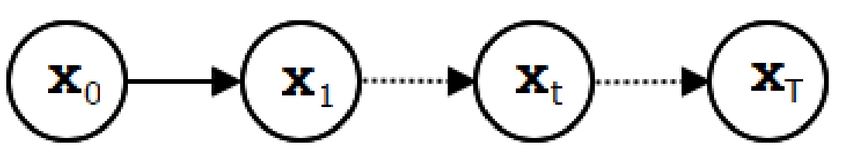
\includegraphics[width=12cm]{images/Reinforcement Learning/markov_chain.png}
    \caption{A Markov chain}
    \label{fig:markov chain}
\end{figure}
Future evolution depends only on the current state $x_{t}$

\subsection{Hidden Markov Models (HMM)}

\begin{figure}[H]
    \centering
    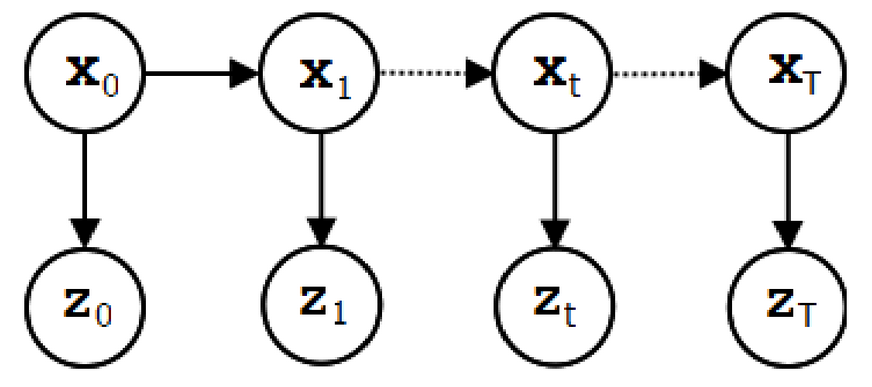
\includegraphics[width=12cm]{images/Reinforcement Learning/hmm.png}
    \caption{An Hidden Markov Model draw}
    \label{fig:hmm}
\end{figure}
states $x_{t}$ are discrete and non-observable, observations (emissions) $z_{t}$ can be either discrete or continuous. Controls $u_{t}$ are not present (i.e., evolution is not controlled by our system).


\textbf{In general}, I cannot observe the state variables $x$, but I can observe the observations $z$ which depends on the observations.

It is a Markov model because is a Markov chain and is hidden because we cannot observe the real state.

\subsubsection{Formal definition}
HMM $= \langle X, Z, \pi_{0} \rangle$ where
\begin{itemize}
    \item transition model: $P(x_{t}|x_{t-1})$
    \item observation model: $P(z_{t}|x_{t})$
    \item initial distribution: $\pi_{0}$
\end{itemize}

the state transition matrix $A = \{A_{ij}\}$
\begin{equation}
    A_{ij} \equiv P(x_{t} = j | x_{t - 1} = i)
\end{equation}

Observation model (discrete or continuous):
\begin{equation}
    b_{k}(z_{t}) \equiv P(z_{t} | x_{t} = k)
\end{equation}
Initial probabilities:
\begin{equation}
    \pi_{0} = P(x_{0})
\end{equation}

\subsubsection{HMM properties and formulae}

We apply the chain rule on HMM:
\begin{equation}
    P(x_{0:T}, z_{0:T}) = P(x_{0})P(x_{1}|x_{0})P(z_{1}|x_{1})P(x_{2}|x_{1})P(z_{2}|x_{2})\dots
\end{equation}

Given a series of observations, we want to determine the distribution over states at some time stamp. Concretely, we want to determine $P(X_{x}|z_{1},z_{2},\dots,z_{n})$. The task is called filtering if $t=n$, smoothing if $t<n$
Given HMM $= \langle X, Z, \pi_{0} \rangle$,
\begin{itemize}
    \item \textbf{Filtering}: $P(x_{T} = k | z_{1:T}) = \frac{\alpha_{T}^{k}}{\sum_{j}\alpha_{T}^{j}}$
    \item \textbf{Smoothing}: $P(x_{t} = k | z_{1:T}) = \frac{\alpha_{t}^{k}\beta^{k}_{t}}{\sum_{j}\alpha_{t}^{j} \beta^{j}_{t}}$
\end{itemize}
where:
\begin{itemize}
    \item forward iterative steps to compute
        \begin{equation}
            \alpha^{k}_{t} \equiv P(x_{t} = k, z_{1:t})
        \end{equation}
        \begin{itemize}
            \item for each state k do: $\alpha^{k}_{0} = \pi_{0}b_{k}(z_{0})$
            \item for each time $t = 1, \dots, T$ do:
            \begin{itemize}
                \item for each state k do:
                \begin{equation}
                    \alpha^{k}_{t} = b_{k}(z_{t}) \sum_{j} \alpha_{t-1}^{j}A_{jk}
                \end{equation}
            \end{itemize}
        \end{itemize}
        
    \item Backward iterative steps to compute
        \begin{equation}
            \beta^{k}_{t} \equiv P(z_{t+1:T}| x_{t} = k)
        \end{equation}
        \begin{itemize}
            \item for each state k do: $\beta^{k}_{T} = 1$
            \item for each time $t = T-1, \dots, 1$ do:
            \begin{itemize}
                \item for each state k do:
                \begin{equation}
                    \alpha^{k}_{t} = \sum_{j} \beta_{t+1}^{j}A_{jk}b(z_{t+1})
                \end{equation}
            \end{itemize}
        \end{itemize}
\end{itemize}


\subsubsection{learning in HMM}

Given output sequences, determine maximum likelihood estimate of the parameters of the HMM (transition and emission probabilities).

\begin{itemize}
    \item \textbf{Case 1}: states can be observed at training time. Note, we are assuming that during training we can see the model. In this case transition and observation models can be estimated with statistical analysis.
    \begin{figure}[H]
        \centering
        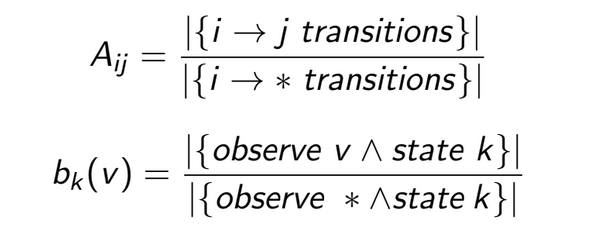
\includegraphics[width=12cm]{images/Reinforcement Learning/case1hmm.png}
        \label{fig:case1hmm}
    \end{figure}

    \item \textbf{Case 2}: states cannot be observed at training time. in this case compute a local maximum likelihood with an Expectation-Maximization (EM) method.
\end{itemize}

\subsection{POMDP agent}

Combines decision making of MDP and non-observability of HMM. We are introducing actions in HMM and we cannot observe states like in MDP.

\begin{figure}[H]
    \centering
    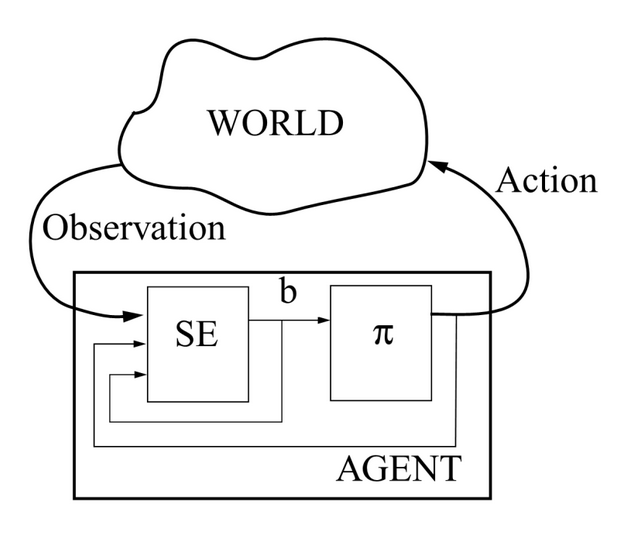
\includegraphics[width=12cm]{images/Reinforcement Learning/POMDP.png}
    \label{fig:pomdp}
\end{figure}

the POMDP representation is $POMDP = \langle X, A, Z, \delta, r, o\rangle$:
\begin{itemize}
    \item X is a set of states
    \item A is a set of actions
    \item Z is a set of observations
    \item $P(x_{0})$ is a probability distribution of the initial state
    \item $\delta(x, a, x') = P(x'|x, a)$ is a probability distribution over transitions
    \item r(x, a) is a reward function
    \item $o(x', a, z') = P(z'|x', a)$ is a probability distribution over observations.
\end{itemize}

the solution of the model is a policy (which is a functions from states to actions like in MDP), but we do not know the states.
The solution can then be a function that maps a set of observations to an action. however is difficult to learn a function that maps observations to actions as observations are potentially infinite. What we can add is the concept of \textbf{belief} of observation.

\subsection{Belief MDP}
we can add concept of belief and learn a function from belief space to actions space.
Belief $b(x) =$ probability distribution over the states. POMDP can be described as an MDP in the belief states, but belief states are infinite.
The set of possible belief is \textbf{exponential} wrt the number of states.

It is possible to transform the POMDP into an MDP, but it is not practical as it moves the model in a very complex space. However there are methods that approximates an MDP. We can use parametric models or piecewise linears to approximate the real transformation and make the POMDP algorithm more efficient.







